\chapter{Fiches Mémotechniques « Haute Rentabilité »}

Ces fiches condensent les faits institutionnels, les dates, les chiffres vérifiés (état au 23 septembre 2026) et les concepts indispensables pour l'épreuve écrite et l'entretien oral. Les mentions « à vérifier » signalent les points que les sources publiques ne permettent pas de confirmer avec certitude : les formuler avec prudence dans la copie.

% =========================================================================
\section{Fiche 1 : Organisation du Ministère (MAECAME)}
% =========================================================================

\begin{tcolorbox}[colback=gray!5!white,colframe=gray!75!black,title=\textbf{Carte d'identité du ministère}]
\begin{itemize}
    \item \textbf{Dénomination :} Ministère des Affaires Étrangères, de la Coopération Africaine et des Marocains Résidant à l'Étranger. Créé par le dahir n° 1-56-097 du 26 avril 1956, au lendemain de l'indépendance. Siège : avenue Franklin Roosevelt, Rabat.
    \item \textbf{Ministre :} M. Nasser Bourita, depuis le 5 avril 2017, reconduit lors du remaniement du 23 octobre 2024 (gouvernement Akhannouch II). Le gouvernement est sortant depuis les législatives du 23 septembre 2026 : ne pas anticiper la composition du prochain exécutif.
    \item \textbf{Portefeuille des MRE :} intégré au ministère depuis la suppression du ministère délégué (2019) ; il n'y a pas de ministre délégué ni de secrétaire d'État chargé des MRE dans le gouvernement Akhannouch II.
    \item \textbf{Réorganisation 2024 :} décret n° 2.24.957 du 21 novembre 2024 fixant les attributions et l'organisation du ministère : regroupement des directions générales en \textbf{pôles homogènes et complémentaires}, création de nouvelles directions, et transformation de l'Académie Marocaine des Études Diplomatiques (AMED, 2011) en \textbf{Institut Marocain de Formation, de Recherche et d'Études Diplomatiques (IMFRED)}.
    \item \textbf{Statut du personnel :} décret n° 2-04-534 du 29 décembre 2004 portant statut particulier du personnel du ministère, modifié par le décret n° 2.22.680 (accès des ingénieurs diplômés des ENSA au corps des conseillers des affaires étrangères).
    \item \textbf{Réseau diplomatique et consulaire :} environ 104 ambassades et missions permanentes et 53 consulats généraux (plus une antenne). En 2026, 21 nouveaux consuls généraux nommés, soit 35 \% des postes consulaires renouvelés, dont environ 40 \% de femmes.
    \item \textbf{Budget :} PLF 2025 d'environ 4,5 milliards de dirhams (+8,9 \%) selon la presse ; budget 2026 présenté au Parlement en novembre-décembre 2025 autour de \textbf{quatre programmes} : modernisation de l'outil diplomatique, diplomatie économique, action bilatérale et multilatérale, services consulaires et état civil ; \textbf{155 postes budgétaires} créés en 2026 (montant global 2026 : à vérifier).
\end{itemize}
\end{tcolorbox}

\begin{tcolorbox}[colback=blue!5!white,colframe=blue!75!black,title=\textbf{Les grandes familles de structures à connaître}]
\begin{itemize}
    \item \textbf{Pôles géographiques et bilatéraux :} Afrique, Europe, Amériques, Asie-Océanie, monde arabe et islamique ; ils pilotent les relations avec chaque pays.
    \item \textbf{Pôle multilatéral et organisations internationales :} ONU et ses agences, Union Africaine, Ligue arabe, OCI, Union pour la Méditerranée, francophonie.
    \item \textbf{Direction de la Diplomatie Économique :} promotion des investissements, des exportations et du « made in Morocco », appui aux entreprises marocaines à l'international, en lien avec l'AMDIE.
    \item \textbf{Coopération africaine et internationale :} en lien avec l'\textbf{AMCI} (Agence Marocaine de Coopération Internationale, 1986), qui gère les bourses des étudiants africains (environ 12 000 boursiers en 2019-2020, 85 \% des étudiants africains boursiers relevant de l'AMCI) et la coopération technique Sud-Sud.
    \item \textbf{Direction des Affaires Consulaires et Sociales (DACS) :} état civil, passeports et documents, protection des Marocains à l'étranger, affaires sociales et juridiques ; source des statistiques consulaires.
    \item \textbf{Direction Générale des Affaires Administratives et Générales :} ressources humaines, budget, moyens généraux et, depuis le décret 2.24.957, une \textbf{Direction des Systèmes d'Information} chargée d'élaborer et d'exécuter les plans du ministère en matière de systèmes d'information, de gérer l'infrastructure et de garantir la cybersécurité. C'est la structure d'accueil naturelle des ingénieurs recrutés.
    \item \textbf{Formation :} IMFRED (ex-AMED), qui forme les diplomates et mène études et recherches.
    \item \textbf{Écosystème des MRE :} Conseil de la Communauté Marocaine à l'Étranger (CCME, créé en 2007, institution constitutionnelle, article 163), Fondation Hassan II pour les MRE (1990), Fondation Mohammed V pour la Solidarité (opération Marhaba), et la future \textbf{Fondation Mohammedia des MRE} annoncée par le Discours de la Marche Verte du 6 novembre 2024.
\end{itemize}
\textit{Note : l'organigramme complet est publié sur }\texttt{diplomatie.ma/fr/structure}\textit{ ; ne citer que les intitulés dont on est sûr (DACS, Direction de la Diplomatie Économique, Direction des Systèmes d'Information, IMFRED).}
\end{tcolorbox}

\IfFileExists{images/img_010_maecame_poles_organigramme.png}{%
\begin{figure}[H]
    \centering
    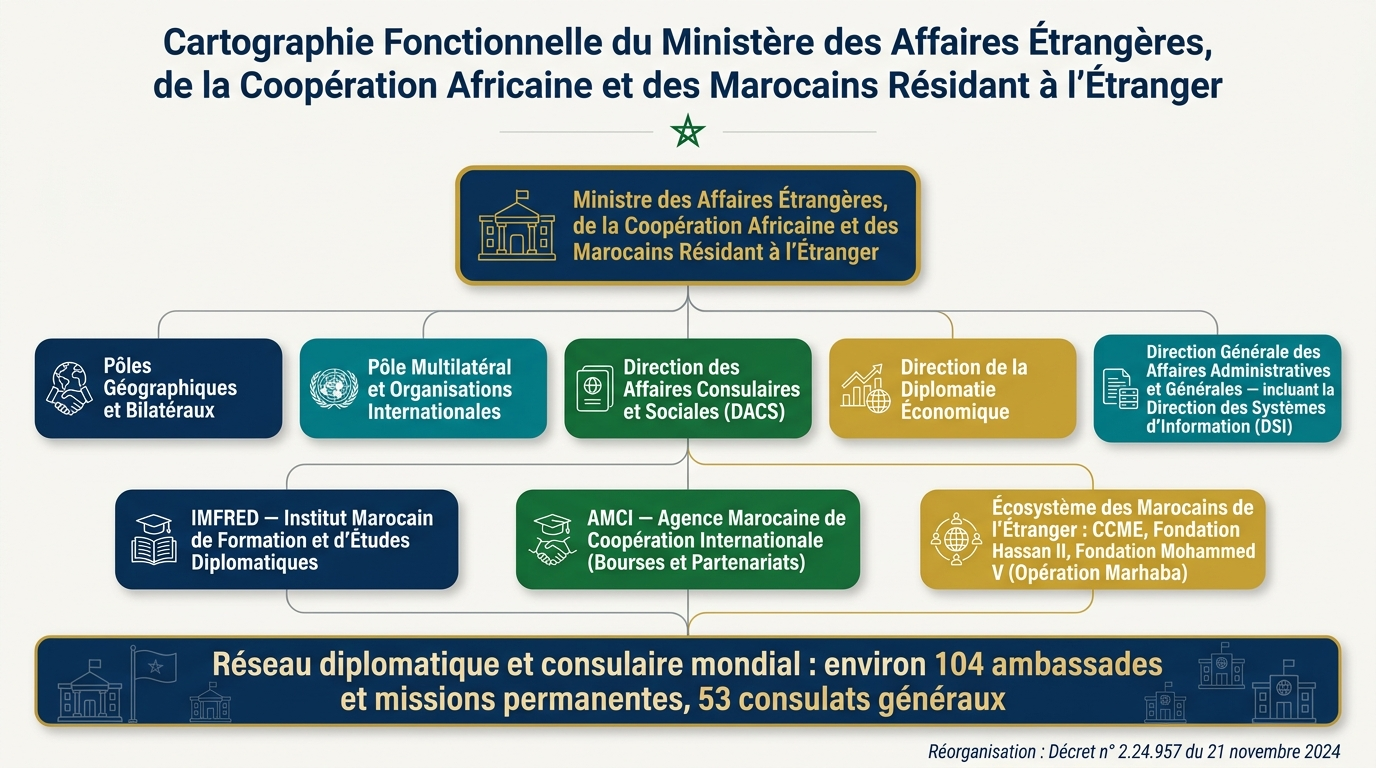
\includegraphics[width=\textwidth]{images/img_010_maecame_poles_organigramme.png}
    \caption{Cartographie fonctionnelle du MAECAME et de son écosystème}
\end{figure}}{}

% =========================================================================
\section{Fiche 2 : Les Constantes de la Politique Étrangère du Royaume}
% =========================================================================

\begin{enumerate}
    \item \textbf{Le Roi, chef de la diplomatie :} la Constitution de 2011 confie au Roi la représentation de l'État et la signature des traités (article 55) ; le préambule affirme l'appartenance du Maroc à l'Afrique, au monde arabo-islamique et à la Méditerranée, et son ouverture sur l'Europe et le monde.
    \item \textbf{La cause nationale :} l'intégrité territoriale et le dossier du Sahara marocain constituent « le prisme » à travers lequel le Royaume évalue ses partenariats (Discours de la Marche Verte 2022).
    \item \textbf{L'ancrage africain :} retour à l'Union Africaine (30 janvier 2017), diplomatie de coopération Sud-Sud, co-développement, Initiative Atlantique, gazoduc Nigeria-Maroc, Fondation Mohammed VI des Oulémas Africains, leadership royal sur la question migratoire.
    \item \textbf{La diversification des partenariats :} Europe (partenaire historique), États-Unis (allié majeur non-OTAN), Chine (partenariat stratégique 2016, Nouvelles Routes de la Soie), monde arabe et pays du Golfe, Amérique latine et Asie.
    \item \textbf{La diplomatie économique :} promotion des investissements, des exportations et de l'image du Royaume (Mondial 2030, énergies renouvelables, hydrogène vert, automobile, Tanger Med, port Dakhla Atlantique).
    \item \textbf{Le multilatéralisme et la crédibilité :} respect du droit international, contribution aux opérations de paix, présidence du Conseil des droits de l'homme en 2024, Pacte de Marrakech sur les migrations (2018), candidature au Conseil de sécurité pour 2028-2029.
    \item \textbf{La diplomatie de proximité :} protection et accompagnement des Marocains du monde, considérés comme partie intégrante de la Nation (articles 16 à 18 de la Constitution).
\end{enumerate}

\IfFileExists{images/img_004_constantes_politique_etrangere.png}{%
\begin{figure}[H]
    \centering
    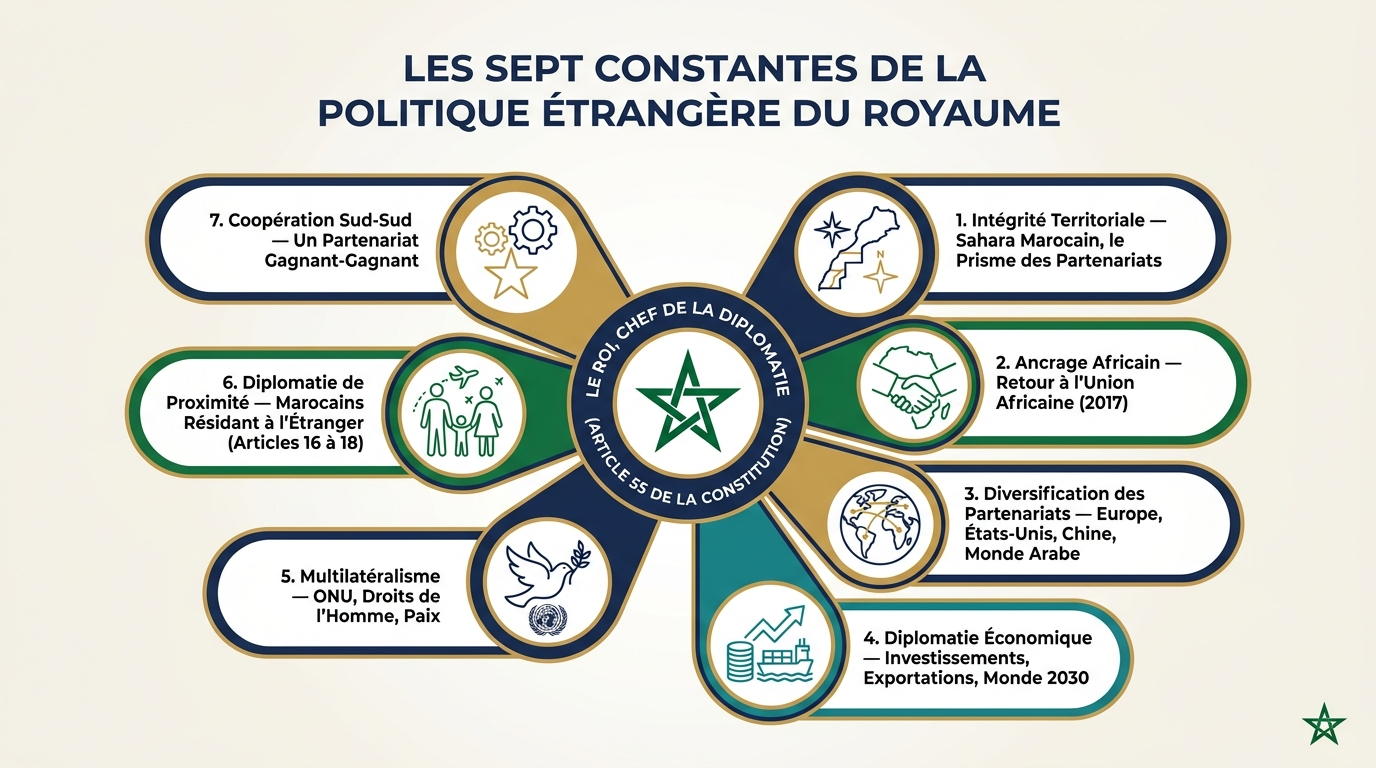
\includegraphics[width=\textwidth]{images/img_004_constantes_politique_etrangere.png}
    \caption{Les sept constantes de la politique étrangère du Royaume}
\end{figure}}{}

% =========================================================================
\section{Fiche 3 : Le Dossier du Sahara Marocain --- Chronologie et Position Internationale}
% =========================================================================

\begin{table}[H]
\centering
\small
\begin{tabular}{|p{3cm}|p{12.5cm}|}
\hline
\rowcolor{gray!20} \textbf{Date} & \textbf{Événement} \\ \hline
6 nov. 1975 & Marche Verte : 350 000 volontaires ; accords de Madrid (14 nov. 1975). \\ \hline
1991 & Cessez-le-feu et création de la MINURSO (Mission des Nations Unies pour l'organisation d'un référendum au Sahara occidental). \\ \hline
11 avril 2007 & Le Maroc présente l'\textbf{Initiative marocaine pour la négociation d'un statut d'autonomie} de la région du Sahara, qualifiée depuis de « sérieuse et crédible » par le Conseil de sécurité. \\ \hline
2015-2016 & Nouveau modèle de développement des provinces du Sud (77 milliards de dirhams), Discours de Laâyoune (6 nov. 2015). \\ \hline
10 déc. 2020 & Proclamation américaine reconnaissant la souveraineté du Maroc sur le Sahara ; réaffirmée par le secrétaire d'État Marco Rubio le 8 avril 2025. \\ \hline
18 mars 2022 & L'Espagne qualifie le plan d'autonomie de « base la plus sérieuse, réaliste et crédible » (lettre du président Sánchez). \\ \hline
30 juillet 2024 & Lettre du président Macron : « le présent et l'avenir du Sahara occidental s'inscrivent dans le cadre de la souveraineté marocaine » ; position réitérée devant le Parlement marocain le 29 octobre 2024. \\ \hline
1\textsuperscript{er} juin 2025 & Le Royaume-Uni juge le plan d'autonomie « la base la plus crédible, viable et pragmatique » (déclaration Lammy-Bourita). \\ \hline
31 oct. 2025 & \textbf{Résolution 2797} du Conseil de sécurité (11 voix pour, 3 abstentions : Chine, Russie, Pakistan ; l'Algérie ne participe pas au vote) : l'autonomie sous souveraineté marocaine est \textbf{la base} des négociations, « solution la plus réalisable » ; mandat de la MINURSO prorogé jusqu'au 31 octobre 2026. \\ \hline
29 janv. 2026 & 15\textsuperscript{e} Conseil d'association Maroc-UE : première position commune des 27 en faveur du plan d'autonomie, confirmée à Rabat le 16 avril 2026 par la Haute Représentante Kaja Kallas. \\ \hline
Fév. 2026 & Réunions de Madrid (8 février) puis de \textbf{Washington (23-24 février)} entre le Maroc, l'Algérie, la Mauritanie et le Polisario, sous l'égide des États-Unis et de l'Envoyé personnel Staffan de Mistura : premiers échanges directs depuis environ sept ans. \\ \hline
22 sept. 2026 & À l'Assemblée générale de l'ONU, M. Bourita énonce \textbf{six principes} (aucune solution hors de l'autonomie sous souveraineté marocaine ; négociation onusienne sur la seule base de l'initiative ; obligations de la résolution 2797 non négociables ; refus du statu quo ; crédibilité liée au respect du cessez-le-feu ; libération des populations de Tindouf). Prochaine échéance : nouvelle résolution avant le 31 octobre 2026. \\ \hline
\end{tabular}
\caption{Chronologie utile du dossier du Sahara marocain}
\end{table}

\IfFileExists{images/img_005_sahara_chronologie_soutiens.png}{%
\begin{figure}[H]
    \centering
    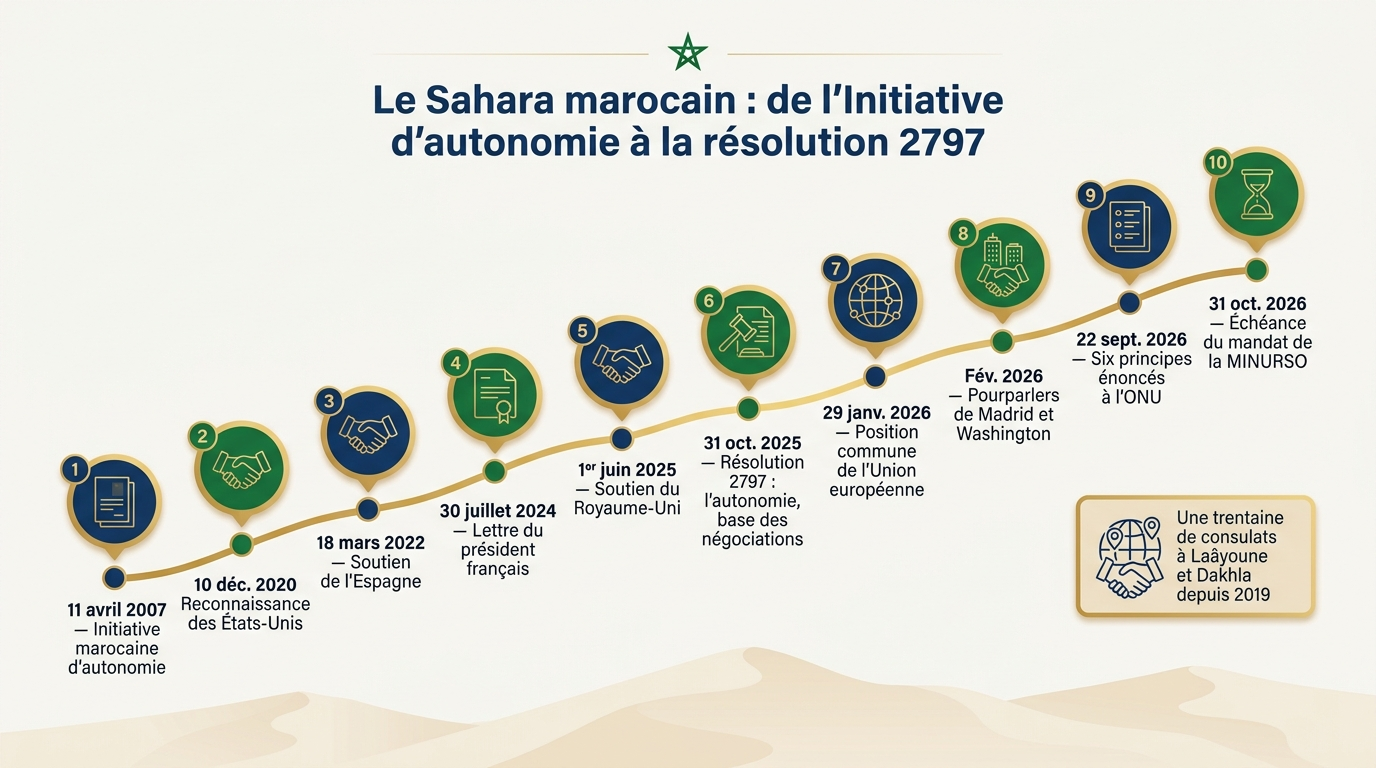
\includegraphics[width=\textwidth]{images/img_005_sahara_chronologie_soutiens.png}
    \caption{Frise du dossier du Sahara : de l'Initiative d'autonomie (2007) à la résolution 2797 (2025)}
\end{figure}}{}

% =========================================================================
\section{Fiche 4 : L'Ancrage Africain et les Grands Projets Structurants}
% =========================================================================

\begin{itemize}
    \item \textbf{Union Africaine :} retour du Maroc le 30 janvier 2017 (après 33 ans d'absence de l'OUA/UA depuis 1984). Demande d'adhésion à la \textbf{CEDEAO} le 24 février 2017, accord de principe le 4 juin 2017, toujours en attente.
    \item \textbf{Migration :} Sa Majesté le Roi désigné « Leader de l'Union Africaine sur la question de la migration » (janvier 2018) ; Pacte mondial de Marrakech (10-11 décembre 2018) ; \textbf{Observatoire Africain des Migrations} inauguré à Rabat le 18 décembre 2020.
    \item \textbf{Initiative Atlantique (novembre 2023) :} offrir aux pays du Sahel (Mali, Burkina Faso, Niger, Tchad) un accès à l'océan Atlantique via les infrastructures marocaines, notamment le \textbf{port Dakhla Atlantique} (environ 1,2 milliard d'euros, livraison attendue en 2028-2029).
    \item \textbf{Gazoduc Nigeria-Maroc (Gazoduc Africain Atlantique) :} environ 6 900 km, 25 milliards de dollars, 13 pays traversés ; accord intergouvernemental signé par les États de la CEDEAO au sommet de Freetown le 19 juillet 2026 ; décision finale d'investissement attendue, premier gaz vers 2031.
    \item \textbf{Coopération Sud-Sud :} AMCI (bourses, formation, expertise), OCP Africa et engrais, Banques marocaines présentes dans une trentaine de pays africains, Royal Air Maroc, Fondation Mohammed VI des Oulémas Africains (dahir du 24 juin 2015, 48 sections nationales fin 2024), Institut Mohammed VI de formation des imams.
    \item \textbf{ZLECAf :} Zone de libre-échange continentale africaine (accord de Kigali, 2018 ; entrée en vigueur 2019) ; le Maroc l'a ratifiée et y voit un levier d'intégration industrielle.
    \item \textbf{Coupe du monde 2030 :} attribuée le 11 décembre 2024 au trio Maroc-Espagne-Portugal (13 juin -- 21 juillet 2030), vitrine de la diplomatie sportive et économique.
\end{itemize}

\IfFileExists{images/img_006_afrique_initiative_atlantique_gazoduc.png}{%
\begin{figure}[H]
    \centering
    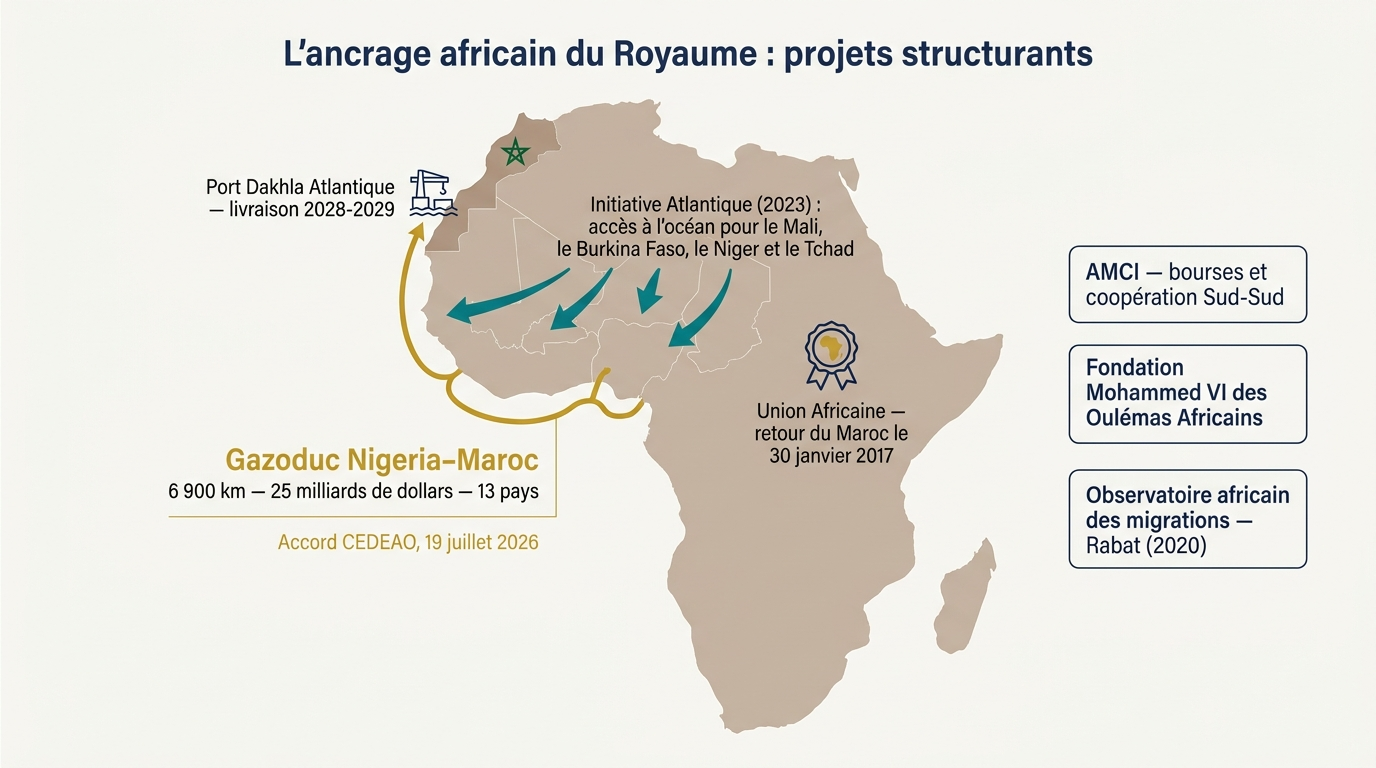
\includegraphics[width=\textwidth]{images/img_006_afrique_initiative_atlantique_gazoduc.png}
    \caption{Carte des projets structurants de l'ancrage africain : Initiative Atlantique et gazoduc Nigeria--Maroc}
\end{figure}}{}

% =========================================================================
\section{Fiche 5 : Les Marocains du Monde --- Chiffres et Politique Publique}
% =========================================================================

\begin{table}[H]
\centering
\small
\begin{tabular}{|p{5cm}|p{4cm}|p{6.5cm}|}
\hline
\rowcolor{gray!20} \textbf{Indicateur} & \textbf{Valeur} & \textbf{Observation} \\ \hline
Effectif des MRE & « Plus de 5 millions » & Chiffre officiel prudent ; la presse évoque souvent 6 millions. Seule statistique exacte : les immatriculés consulaires. \\ \hline
Transferts 2024 & 117,7 MMDH (+2,1 \%) & Soit 7,7 \% du PIB ; ils étaient de 57,4 MMDH en 2014 (doublement en dix ans). \\ \hline
Transferts 2025 & Plus de 122 MMDH (+2,6 \%) & Première source de devises avec le tourisme et les phosphates ; stabilisent les réserves de change. \\ \hline
Transferts à fin juillet 2026 & 74,78 MMDH (+8,1 \%) & Dynamique soutenue en 2026. \\ \hline
Opération Marhaba 2026 & 4 137 594 MRE accueillis (+1,8 \%) & Du 10 juin au 15 septembre ; 26 espaces d'accueil, 1 134 assistantes sociales, pics d'environ 80 000 arrivées par jour (Fondation Mohammed V pour la Solidarité). \\ \hline
Participation politique 2026 & Vote par procuration dématérialisé & Plateforme « E-procuration » (24 août -- 22 septembre 2026) ; pas de bureaux de vote à l'étranger ni de sièges réservés. \\ \hline
\end{tabular}
\caption{Tableau de bord des Marocains du monde}
\end{table}

\begin{tcolorbox}[colback=yellow!5!white,colframe=orange!75!black,title=\textbf{La réforme des institutions des MRE (Discours de la Marche Verte, 6 novembre 2024)}]
\begin{itemize}
    \item \textbf{Constat royal :} dispersion des intervenants, résultats insuffisants malgré les moyens ; nécessité d'une « refonte globale ».
    \item \textbf{Deux piliers :} (1) le \textbf{CCME} recentré sur la réflexion stratégique et la prospective ; (2) une nouvelle \textbf{Fondation Mohammedia des MRE}, bras opérationnel qui regroupe les attributions dispersées (dont celles de la Fondation Hassan II).
    \item \textbf{Mécanisme national de mobilisation des compétences} des Marocains du monde (médecins, ingénieurs, chercheurs, entrepreneurs) au service du développement.
    \item \textbf{État d'avancement :} en septembre 2026, les textes créant la Fondation n'ont pas encore été adoptés : parler d'une réforme « en cours de mise en œuvre ».
    \item \textbf{Cadre constitutionnel :} articles 16 (protection des droits et intérêts des MRE), 17 (droits de citoyenneté, dont le vote) et 18 (participation aux institutions consultatives) de la Constitution de 2011.
\end{itemize}
\end{tcolorbox}

\IfFileExists{images/img_007_mre_transferts_marhaba_reforme.png}{%
\begin{figure}[H]
    \centering
    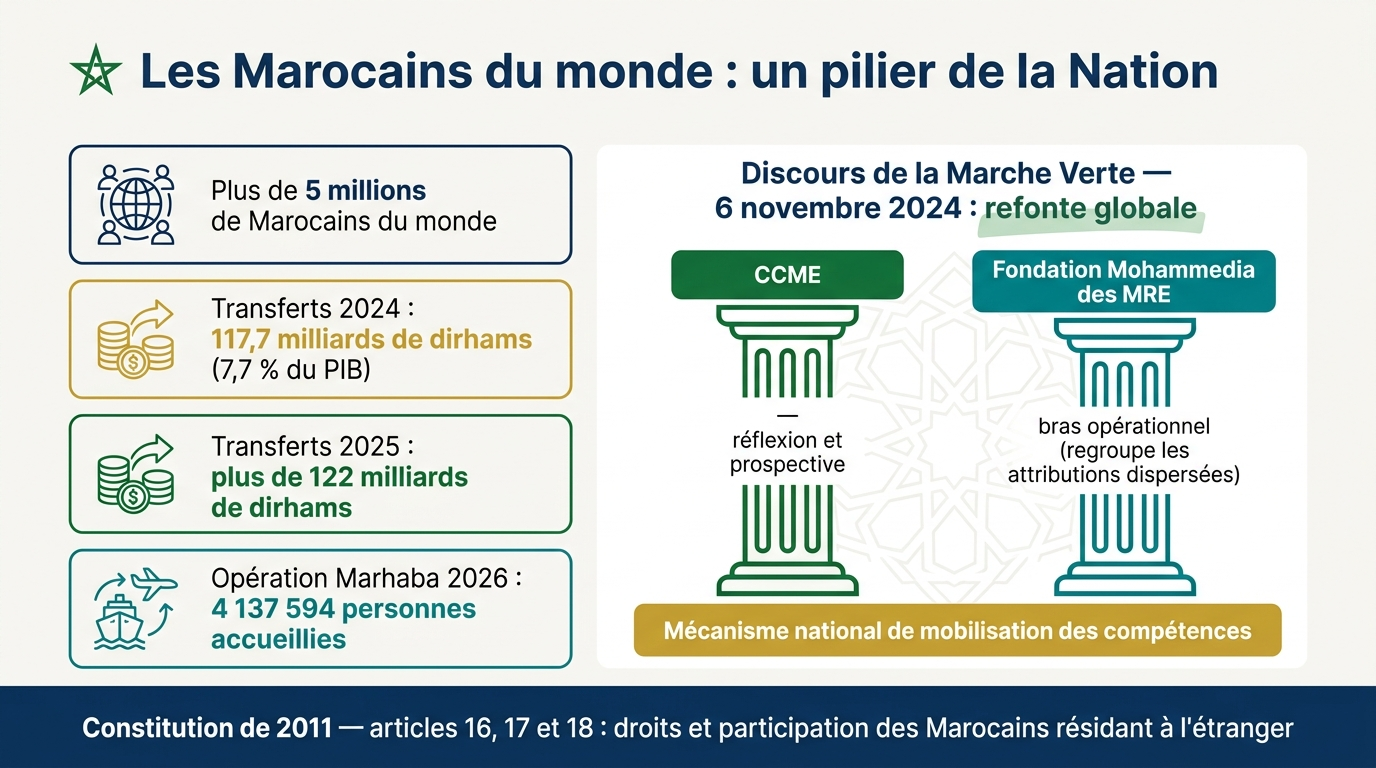
\includegraphics[width=\textwidth]{images/img_007_mre_transferts_marhaba_reforme.png}
    \caption{Marocains du monde : transferts, opération Marhaba et refonte institutionnelle}
\end{figure}}{}

% =========================================================================
\section{Fiche 6 : Partenariats Stratégiques et Actualité 2024-2026}
% =========================================================================

\begin{itemize}
    \item \textbf{Union européenne :} premier partenaire commercial ; statut avancé (2008). Arrêt de la Cour de justice de l'UE du 4 octobre 2024 annulant les accords agricole et de pêche ; nouvel accord agricole par échange de lettres publié au Journal officiel de l'UE le 3 octobre 2025 (application provisoire) ; pas de nouvel accord de pêche à ce jour. Position commune des 27 sur l'autonomie (janvier 2026).
    \item \textbf{États-Unis :} accord de libre-échange (2006), allié majeur non-OTAN, exercice African Lion, reconnaissance de la souveraineté sur le Sahara (2020, réaffirmée en 2025), médiation des pourparlers de Washington (février 2026).
    \item \textbf{Espagne et France :} partenaires historiques ; co-organisation du Mondial 2030 avec l'Espagne ; visite d'État du président Macron (octobre 2024) et « partenariat d'exception renforcé ».
    \item \textbf{Israël :} déclaration tripartite du 22 décembre 2020 ; le 16 septembre 2026 à New York, accord pour élever les bureaux de liaison au rang d'\textbf{ambassades} et échanger des ambassadeurs, avec accords d'investissement et de double imposition avant fin 2026. Le Maroc défend l'État palestinien dans les frontières de 1967 avec Al-Qods-Est pour capitale et préside le Comité Al-Qods.
    \item \textbf{Gaza :} accord de participation du Maroc à la Force internationale de stabilisation signé à Rabat le 15 juillet 2026 ; Maroc membre fondateur du Conseil de paix.
    \item \textbf{Chine :} partenariat stratégique (mai 2016), premier pays maghrébin signataire des Nouvelles Routes de la Soie (novembre 2017), plan de mise en œuvre conjoint (5 janvier 2022) ; investissements dans l'automobile électrique et les batteries.
    \item \textbf{Algérie :} rupture des relations diplomatiques le 24 août 2021, fermeture de l'espace aérien (septembre 2021), non-renouvellement du gazoduc Maghreb-Europe (octobre 2021), frontières terrestres fermées depuis 1994 ; présence algérienne aux pourparlers de 2026. Position marocaine constante : la main tendue (discours royaux de 2018, 2021 et 2022).
    \item \textbf{Multilatéral :} membre du Conseil des droits de l'homme 2023-2025, \textbf{présidence en 2024} (ambassadeur Omar Zniber) ; candidature au \textbf{Conseil de sécurité 2028-2029} (dernier mandat 2012-2013), soutenue par le Sommet arabe de Bagdad (mai 2025).
\end{itemize}

% =========================================================================
\section{Fiche 7 : Le Numérique au Service de la Diplomatie et des Services Consulaires}
% =========================================================================

\begin{itemize}
    \item \textbf{e-Visa :} lancé le 10 juillet 2022 (plateforme acces-maroc.ma) ; visa électronique en 72 heures (24 heures en express), valable 30 jours ; \textbf{385 738 e-visas} délivrés à fin 2024, à 95 \% pour le tourisme, 111 nationalités (l'Inde en tête).
    \item \textbf{Services consulaires en ligne :} portail \texttt{consulat.ma} (guide des services), \texttt{rdv.consulat.ma} (prise de rendez-vous), plateforme interne \textbf{eConsulat} enrichie de nouveaux modules (rapatriement des dépouilles, authentification des permis de conduire, échanges avec le ministère de la Justice) ; objectif de temps d'attente ramené de 45 minutes (2025) à 38 minutes (2026).
    \item \textbf{Apostille :} adhésion du Maroc à la Convention de La Haye (en vigueur le 14 août 2016), demande en ligne sur \texttt{apostille.ma} : simplification de la légalisation des documents pour les MRE et les investisseurs.
    \item \textbf{Cadre de sécurité :} loi 05-20 sur la cybersécurité et son décret 2-21-406 (15 juillet 2021) ; DGSSI (Administration de la Défense Nationale) ; \textbf{Stratégie nationale de cybersécurité 2030} (juillet 2024 : 4 piliers, 11 objectifs, 26 initiatives, 60 actions) ; loi 09-08 et CNDP pour les données personnelles, particulièrement sensibles pour un réseau de 150 postes à l'étranger.
    \item \textbf{Enjeux pour l'ingénieur d'État :} interopérabilité entre consulats, état civil et administrations nationales (RNP, Justice, Intérieur), continuité de service sur des fuseaux horaires multiples, protection des données des Marocains du monde, lutte contre la fraude documentaire (biométrie), communication numérique et image du Royaume, données au service de la diplomatie économique.
\end{itemize}

\IfFileExists{images/img_008_services_consulaires_numeriques.png}{%
\begin{figure}[H]
    \centering
    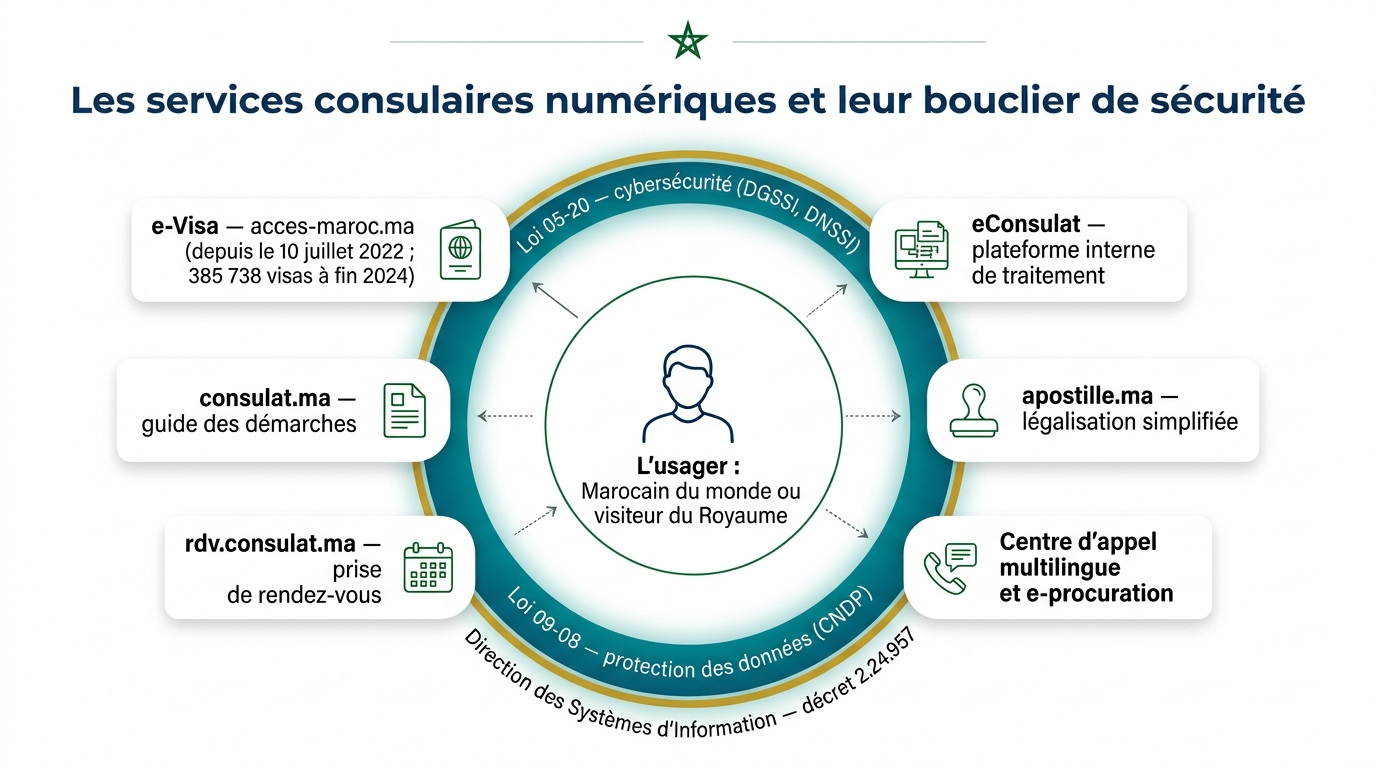
\includegraphics[width=\textwidth]{images/img_008_services_consulaires_numeriques.png}
    \caption{Écosystème numérique des services consulaires : e-Visa, eConsulat, apostille et sécurité des données}
\end{figure}}{}

% =========================================================================
\section{Fiche 8 : Chiffres et Dates à Retenir par Cœur}
% =========================================================================

\begin{multicols}{2}
\small
\begin{itemize}
    \item \textbf{1956 :} création du ministère.
    \item \textbf{1975 :} Marche Verte (6 novembre).
    \item \textbf{1984 :} retrait de l'OUA ; \textbf{2017 :} retour à l'UA (30 janvier).
    \item \textbf{2007 :} Initiative d'autonomie (11 avril) ; création du CCME.
    \item \textbf{2011 :} Constitution (articles 16-18 sur les MRE, article 55 sur les traités).
    \item \textbf{2016 :} partenariat stratégique avec la Chine ; apostille en vigueur.
    \item \textbf{2018 :} Pacte de Marrakech sur les migrations ; Roi leader UA migration.
    \item \textbf{2020 :} reconnaissance américaine (10 décembre) ; Observatoire africain des migrations (18 décembre).
    \item \textbf{2022 :} lancement de l'e-Visa (10 juillet) ; Espagne soutient l'autonomie.
    \item \textbf{2023 :} Initiative Atlantique (novembre).
    \item \textbf{2024 :} lettre Macron (30 juillet) ; présidence du CDH ; décret 2.24.957 de réorganisation ; Discours MRE (6 novembre) ; Mondial 2030 attribué (11 décembre).
    \item \textbf{2025 :} Royaume-Uni (1\textsuperscript{er} juin) ; résolution 2797 (31 octobre) ; transferts MRE $>$ 122 MMDH.
    \item \textbf{2026 :} position UE (29 janvier) ; pourparlers de Washington (février) ; accord gazoduc CEDEAO (19 juillet) ; ambassades Maroc-Israël (16 septembre) ; six principes à l'ONU (22 septembre) ; échéance MINURSO (31 octobre).
    \item \textbf{Réseau :} environ 104 ambassades, 53 consulats généraux.
    \item \textbf{MRE :} plus de 5 millions ; 117,7 MMDH en 2024 (7,7 \% du PIB) ; 4,14 millions accueillis par Marhaba 2026.
    \item \textbf{Gazoduc :} 6 900 km, 25 milliards de dollars, 13 pays.
    \item \textbf{e-Visa :} 385 738 délivrés à fin 2024.
\end{itemize}
\end{multicols}
